\chapter{Background}
\label{chap:background}

Education has evolved with culture and technology.  Classical wisdom calls only for the ``three R's" (reading, writing, and arithmetic) in schools, which today is considered foundational but insufficient for life. Education has been expanded to include history, science, advanced mathematics, art, and technology. The current focus on scientific and mathematical education is called ``STEM," referring to Science, Technology, Engineering, and Math. Engineering and technology now aspire to sit with equal prominence as science and math.  This study observes the development of design thinking in middle school students, and investigates a few of the skills necessary to get there.

\section{Brief History of Engineering Education}

STEM education, of which engineering is a component, is in need of ``evidence-based" tools to measure their effectiveness \citep{csed-guzdial}. With that, much of the literature used is from closely related academic fields, specifically science and math education. Despite the larger depth of work in those fields, they all succumb to a problem inherent in education research: there is a disconnect between locally generated and generalizable knowledge. Techniques generated in classrooms that are locally usable and effective often do not translate well to other classroom settings. While that knowledge may work in one circumstance, it is little beyond anecdotal to the greater community. Conversely, lab-generated scientific data on education is often too abstract to be directly usable
for real teachers \citep{sandoval}.

With more emphasis being put on technology in education, the development of computational thinking becomes important \citep{p33-wing}. Computational thinking is the collection of concepts, skills, and abstractions people need to best leverage computers and technology as an aid in human knowledge development. Thinking computationally is difficult, but with it people are able to solve new problems with the help of computation theory. 

\citet{brown-1992} conducted much of her work around the development of a learning community in lieu of the traditional didactic classroom experience. In a traditional environment, students are {}``passive recipients'' of information dispatched by teachers and media. The relationship is largely unidirectional, where the only return of information from the students is from assessments that are
based on drill, practice, and memorization. In this environment the
students needs only to develop skills at storing rote facts and reproducing
them on demand. Such an environment is prime for many pedagogical pitfalls,
such as the development of a disconnect between knowledge and belief,
where students may understand a concept as it was presented but do
not believe it to be true \citep{chinn-samar}. 

In Brown's community of learners, students begin to act as researchers
and co-teachers of the material. The teachers, rather than function
as managers assigning repetitive tasks, become facilitators who present
the tools and encourage the curiosity necessary for engaging learning
experiences. The teacher also serves as a good role model for learners,
who show interest and discovery themselves. A classroom in this mode
is no longer a work camp producing documents, but a research lab motivated
by coherence and deep understanding. Assessments ideally are wrapped
in immersive applications of knowledge such as projects and portfolios
which can be subjectively as well objectively analyzed. 

One of the fundamental skills outlined by Brown is the ability to self-monitor. \citet{atman-1999} support this, claiming self-monitoring to be a critical component of successful students. When a student engages in self-monitoring, the student can identify when he or she is both succeeding and stuck, and takes appropriate actions to reach their learning goal. This skill considered part of meta-cognition, which is an advanced but teachable set of thinking skills \citep{beyer88}.

Strategies that are today considered meta-cognitive appear early and often in education literature. \citet{bloombroder50} describe observed differences between successful and non-successful students as they approach problem solving. Successful students were better at, among other things, understanding problem requirements and maintaining contact with those requirements as they worked towards a solution. This is a fundamental element of self-monitoring.

Meta-cognition is, especially in children, hard to develop. Children empirically do not employ many meta-cognition techniques, if any at all. Most adults do, using strategies to overcome natural limitations of memory retention and recollection \citep{brown-1992}. The process of design has an intrinsic emphasis on meta-cognitive processes, as it has been shown to help students effectively learn about complex systems \citep{designing-to-learn}. The effectiveness of a design process is greatly enhanced by the inclusion of a feedback system, where the designer is re-analyzing both the problem and what he or she has done thus far to approach it. This concept is seen throughout the literature, often citing the ``reflective practitioner" of \citet{schon83}. 

The stages of cognitive development defined by \citet{piaget69} help explain the slow development of metacognitive abilities. Children in middle school are only just entering the formal operations phase where they can perform reasoning on abstract representations. The metacognition skills required in engineering require abstract evaluation. Development of these skills is not possible until the child is cognitively ready, which does not generally happen until 15 to 18 years into life. 

Building on \citet{schon83}, \citet{atman-2003} described iteration as the core tenet of design, triggered by certain cognitive activities: self-monitoring, clarification, and examination. Problem-setting in addition to problem-solving
is emphasized. Reasoning is done through experimentation. A variety
of representations are generated, and fluidly moved between to best
serve the thought of the moment. The reflective practitioner is not
just a developer making a solution, he or she is an experimental scientist
trying to understand the situation he/she created in solution development.
These ideas, executed in tightly iterating loops, are the image of an ideal design strategy as described by \citeauthor{schon83}.

Many researchers and educators have attempted to model the design process. Most of these models have strong thematic similarities, usually including the following states: learning about the problem, identifying resources and constraints, generating ideas, implementation, testing, and revising. Despite the general similarities, different models can communicate completely different methods for design. For one example, \citet{welch} claims that the states of the design process are essentially unordered, allowing the designer to move laterally to any state at any time. On the other hand, \citet{kimbell06} reported upon numerous models that are linear or have a tightly-prescribed progression through steps. The multitude of contrasting views of the design process is currently a source of conflict in the education community \citep{REESE}, and is an important topic of consideration in this research.

\citet{mos-design} created a model designed for use by teachers who may not themselves be trained designers. It is intended to be used as part of a curriculum about design for young students, and may not be based on professional methodology. In this model five states form a ring, where travel is only implied to be possible between adjacent states. The states are Imagine, Plan, Create, Test, and Improve. The literature accompanying this model expresses that the student does not need to be bound by this ring, and may move from any state to any other state at any time. However, the graphic does not represent this and strongly implies the notion of neighbor-only traversal.

\citet{atman-2003} presents a model derived from observations of senior-level undergraduate engineering students. This model %, visualized in Figure \ref{fig:senior-cycle},
is scientifically accurate to an actual process that took place in research subjects. It is both more complex and less beautiful than the Museum of Science model, and is clearly intended for a different audience. Many would argue that the model presented by Adams is more useful, as it represents a functional process, but that depends on the individual's definition of usefulness. To an elementary school teacher, the Museum of Science model, while clearly incomplete, may be the correct tool for the job at hand. 

Most of these models have a heavy emphasis on iteration. \citet{dow09} found that iteration was critical to success of a time-constrained design problem. Participants with no prior experience who iterated through their design process performed as well as the participants who had prior experience but did not iterate. The process of repeating design tasks helped the participant explore the problem space and become familiar with the relevant physics. \citet{eckert09} found that iteration also takes on additional influence in corporate engineering, where a new design can depend on the proven framework of previous designs. 

%\begin{figure}
%\centering
%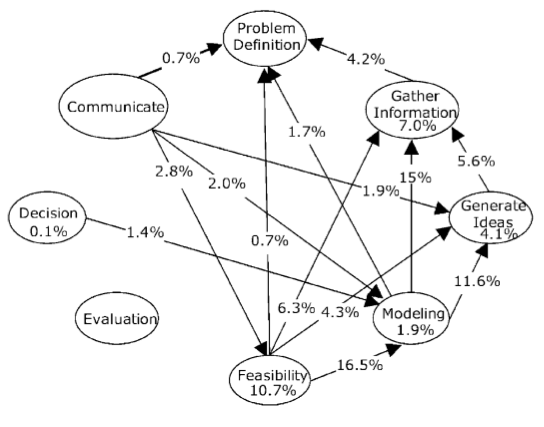
\includegraphics[width=0.85\textwidth]{atman-senior-cycle}
%\caption{\label{fig:senior-cycle}Engineering process as observed in senior
%engineering students \citet{atman-2003}}
%\end{figure}

\section{Design Activity Studies}
	\label{sec:activity-design-studies}
\citet{welch} performed an experiment on design activities
carried out by seventh grade students. In this study, students worked
in dyads to build the tallest paper tower out of a finite set of resources
within a specific time period. Welch enumerated a design process as
five steps that represented a general consensus of concepts available
in literature. The steps are:

\begin{enumerate}
\item Understand the problem
\item Generate possible solutions
\item Model a possible solution
\item Build a solution
\item Evaluate the solution
\end{enumerate}

Welch claimed that the actual process undergone by both professionals
and amateurs of design would not be linear, and that it would recurse
on itself many times. The activity was intended to be representative
of a real-world engineering task, characterized by having a goal,
constraints, and some criteria to recognize a successful solution.
The students worked in pairs, which is also an element of simulating
real-world design, where most development is the result of combined
efforts of two or more people working cooperatively.

Design of activities for this research was also informed by the
model-eliciting activities of \citet{lesh03}. Lesh's work was based in
mathematics education, and this paper used fractions and proportions as the subject
to be explored by the research participants. A model-eliciting activity (MEA) is \label{sec:MEA}
designed such that the students' product is not a single
answer, but a rule or process that can be applied to solve similar
problems. Three MEAs are presented in the cited paper. The simplest example
is the ``bigfoot'' activity, where students are told they are
forensic examiners and need to identify the height of a person based
on a shoe print. The expected response is for students, working in
small groups, to observe themselves, and somehow create a proportion
between human shoe size and height. The students are not requested
to determine the height of the one example person, but to provide
the police with a mechanism with which they can identify the height
of any person based on shoe size. 

The results of the MEA research, besides the concept of the MEA itself,
is that problem solving can be viewed as a process of local concept
development. Many researchers in the past have studied the process
of learning concepts, specifically in math and science. Lesh concluded
that the same process and principles involved in normal concept learning
occur in a fast, recursive fashion during problem solving. The concepts
being developed during problem solving are not necessarily general, they are specific
to the current problem and the situation surrounding it, but the same
development process has been observed. This observation allows the
connection to be drawn between local problem solving and general,
long-term cognitive development.

\section{This Study}
Many studies have examined the design process, providing a variety of insightful models and theories. Some of these studies, such as \citet{schon83} and \citet{eckert09}, model how adult, professional engineers perform design tasks. Others focus on children, like \citet{welch} and \citet{lesh03}. These latter studies provide a look at how students generally go about design tasks, but they do not examine the elements of what makes up a design process. Models such as that presented by \citet{mos-design} provide states of thought that students and professionals alike seem to pass through, but do not investigate the component actions that make that process what it is. 

One of the most fundamental of these components is the process of iteration, about which study has just begun. \citet{dow09} analyzed the increase in efficacy provided by the presence of an iterative process in college students. This study shows that iteration is verifiably critical part of effective design.  %
The author is not aware of any studies that focus on middle school students and the role of iteration in the design process. This study takes this focus, observing and interpreting students' design processes across a variety of problem types.

% Original paragraph continues here.... replaces with above.
%From this platform questions arise about the natural desire and patterns students express towards design iteration. No detailed study on iteration has focused on observation of natural tendencies, nor investigated the middle school age group. The studies that do use that age group do not provide elemental understanding of what drives the student to go through the process models that are presented. No studies presented utilized a variety design problem types. This study fits in this space, having examined middle school students direct interaction with a variety of problems. 

